\chapter{Results and Discussion} % Main chapter title

\label{Chapter 4} % Change X to a consecutive number; for referencing this chapter elsewhere, use \ref{ChapterX}

\lhead{Chapter 4. \emph{Results and Discussion}} % Change X to a consecutive number; this is for the header on each page - perhaps a shortened title

For the evaluation component of our study, we consider both a general-purpose baseline language model and a set of domain-specialized, medically fine-tuned models. As our baseline, we employ Mistral-7B-Instruct-v0.2, a large language model that, while not specifically adapted for medical tasks, has been pretrained on an extensive and diverse corpus. This enables us to benchmark the performance expected from a high-capacity LLM without domain-specific optimization.

To assess the impact of medical fine-tuning, we further include three models that have undergone targeted adaptation for biomedical or clinical applications: Microsoft BioGPT, JSL-Med-Sft-Llama-3-8B, and Apollo. These models allow us to systematically compare the baseline’s general reasoning capabilities against the specialized strengths of medically aligned LLMs. By evaluating both categories side-by-side, we aim to quantify the extent to which domain-specific fine-tuning enhances performance on medical tasks and to better understand the trade-offs between general and specialized model design.

\begin{table}[H]
    \centering
    \begin{tabular}{lcc}
    \toprule
    \textbf{Model} & \textbf{Accuracy (\%)} 
    \\
    \midrule
    Mistral-7B-Instruct-v0.2 & 44 \\
    Microsoft BioGPT & 35 \\
    JSL-Med-Sft-Llama-3-8B & 32 \\
    Apollo & 23 \\
    \bottomrule
    \end{tabular}
    \caption{Diagnostic accuracy of open-source LLMs on AgentClinic.}
\end{table}

\begin{figure}[h!]
    \centering
    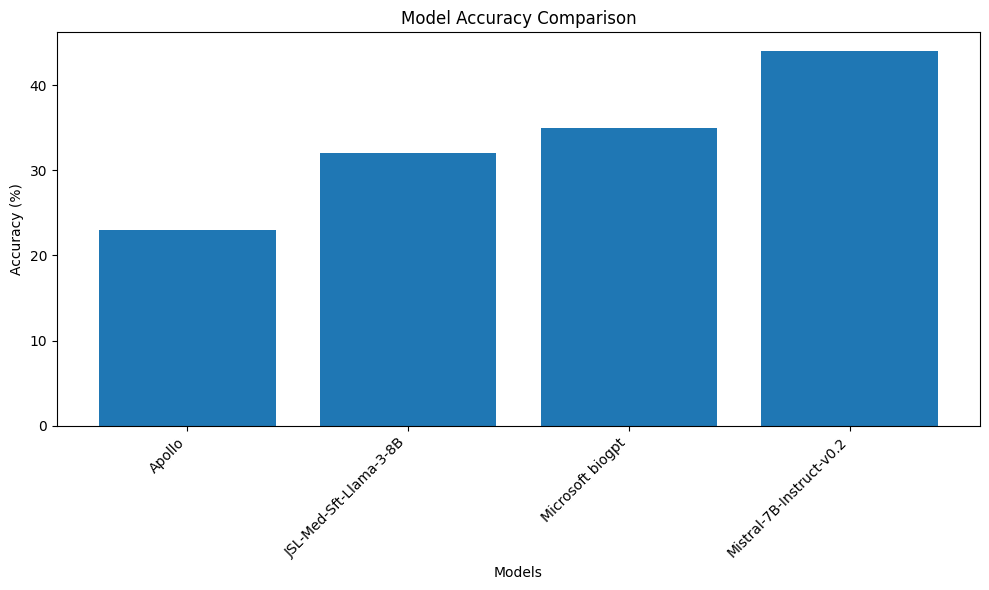
\includegraphics[width=0.7\textwidth]{Pictures/model comparison diks mtp.png}
    \caption{Performance bar chart for models on MedQA dataset.}
    \label{fig:myimage}
\end{figure}


\section{Diagnostic Accuracy Results}
% \textit{(Placeholder: Insert accuracy results for each model here.)}

% \begin{table}[H]
%     \centering
%     \begin{tabular}{lcc}
%     \toprule
%     \textbf{Model} & \textbf{Accuracy (\%)} & \textbf{Notes} \\
%     \midrule
%     Model A & -- & Placeholder \\
%     Model B & -- & Placeholder \\
%     Model C & -- & Placeholder \\
%     \bottomrule
%     \end{tabular}
%     \caption{Diagnostic accuracy of open-source LLMs on AgentClinic.}
% \end{table}

From the comparison of model accuracies, it is clear that different models exhibit varying levels of effectiveness on the given task. The performance trend shows a consistent improvement from general-purpose models toward more specialized or instruction-tuned models. Among all evaluated models, Mistral-7B-Instruct-v0.2 stands out with the highest accuracy, indicating its strong suitability for the problem setting. In contrast, Apollo shows noticeably weaker performance, suggesting that it may not be ideal for similar tasks. The results highlight the importance of model selection based on instruction-tuning quality and domain alignment.

\textbf{Key Observations:}
\begin{itemize}
    \item \textbf{Mistral-7B-Instruct-v0.2 achieves the highest accuracy (44\%):} making it the most reliable model for this task.

    \item Microsoft BioGPT performs strongly (35\%), benefiting from its biomedical specialization.

    \item JSL-Med-Sft-Llama-3-8B shows moderate accuracy (32\%), performing better than Apollo but below BioGPT and Mistral.

    \item Apollo has the lowest accuracy (23\%), suggesting limited suitability for the evaluated task.

    \item Overall trend: Accuracy increases progressively from Apollo → JSL-Med → BioGPT → Mistral.

    \item Performance gap: The top model outperforms the lowest by over 20 percentage points, indicating a substantial difference in capability.
\end{itemize}

\begin{table}[H]
    \centering
    \begin{tabular}{l c p{4.2cm} c p{3.5cm}}
    \toprule
    \textbf{Model} & \textbf{Size} & \textbf{Training Data} & \textbf{Med. FT} & \textbf{Evaluation Data} \\
    \midrule
    Mistral-7B-Instruct-v0.2 & 7B & General instruction-tuning datasets & No & MedQA \\
    Microsoft BioGPT & 1.5B & PubMed abstracts and biomedical literature & Yes & MedQA \\
    JSL-Med-Sft-Llama-3-8B & 8B & Clinical + biomedical SFT dataset (John Snow Labs) & Yes & MedQA \\
    Apollo & 7B & General web + text corpora (non-medical) & No & MedQA \\
    \bottomrule
    \end{tabular}
    \caption{Model details: size, training data, medical fine-tuning status, and evaluation dataset.}
\end{table}

Fine-tuned medical models such as BioGPT and JSL-Med often perform worse than strong pretrained instruction models because they are optimized for narrow biomedical tasks rather than general reasoning or instruction following. This specialization can lead to catastrophic forgetting, where the model loses broad linguistic and reasoning capabilities during domain-specific fine-tuning. \\

Additionally, medical fine-tuning datasets are typically smaller and less diverse, limiting their ability to generalize to tasks like classification or accuracy-based evaluation. In contrast, instruction-tuned models like Mistral-7B-Instruct are trained on large, high-quality datasets designed specifically to improve reasoning, comprehension, and accuracy, enabling them to outperform domain-specific models even on medically oriented tasks.


\section{Bias Impact Analysis}

The results show that introducing cognitive or demographic biases into the diagnostic pipeline significantly reduces the model’s accuracy compared to unbiased conditions. The model performs best when no bias is applied (44\%), highlighting the importance of neutral and consistent input behavior for reliable diagnostic reasoning. \\

Recency bias (34\%) and gender bias (35\%) cause noticeable degradation, suggesting that the model becomes overly influenced by recent cues or demographic cues rather than evaluating clinical evidence holistically. 
Confirmation bias leads to the lowest accuracy (32\%), indicating that once the model forms an early hypothesis, it tends to fixate on supporting evidence and ignore contradictory information. \\

Overall, the analysis emphasizes that biases—whether cognitive or demographic—introduce systematic distortions into LLM-driven diagnostic reasoning and reduce performance in realistic clinical settings. \\
\begin{figure}[h!]
    \centering
    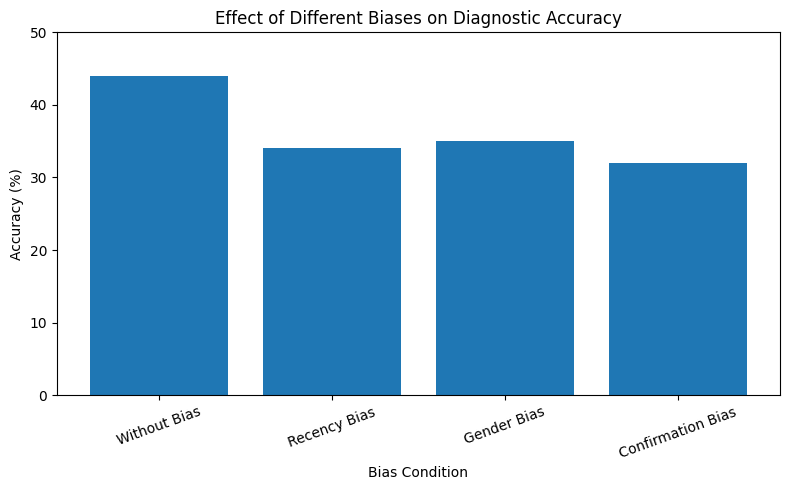
\includegraphics[width=0.7\textwidth]{Pictures/bias effect.png}
    \caption{Effect of bias on model performance.}
    \label{fig:myimage}
\end{figure}

% \section{Qualitative Dialogue Observations}
% \textit{(Placeholder: Add dialogue samples or behavioural notes.)}

% \section{Discussion}
% \textit{(Placeholder: Add analytical discussion based on observed results.)}